\documentclass{beamer}    % 14pt je nenujen
\usepackage[T1]{fontenc}
\usepackage[utf8]{inputenc}
\usepackage[slovene]{babel}
\usepackage{pgfpages}           % privat zapiski
\usepackage{amsfonts}
\usepackage{amsmath,amsthm}     % pravilen izpis v "math mode"
%\usepackage{hyperref}
\usepackage{graphicx}           % za slike
\usepackage{tikz}
\usepackage{multicol}
\usepackage{ulem}
\usepackage{bibentry}
\usepackage{bbm}
\usepackage{algorithm}
\usepackage{algorithmic}

\usepackage{forest,calc}
\forestset{
  make tab/.style args={#1:#2:#3/#4:#5:#6/#7:#8:#9}{%
    content={%
      \tabcolsep=.6\tabcolsep
      \begin{tabular}{p{\widthof{x}}|p{\widthof{x}}|p{\widthof{x}}}
        #1 & #2 & #3\\\hline#4&#5&#6\\\hline#7&#8&#9
      \end{tabular}}},
  label position r/.initial=right,
  label position b/.initial=below
}

%\hypersetup{hidelinks}

\setbeamertemplate{theorems}[ams style]             % numbered da brez bold 

\setbeameroption{hide notes}                        % samo prosojnice
%\setbeameroption{show only notes}                   % samo zapiski
%\setbeameroption{show notes on second screen=right}  % oboje

\usepackage{palatino}
\usefonttheme{serif}

%\usecolortheme{dracula} %ali beetle morda ali seagull 

\setbeamertemplate{navigation symbols}{} % izklop navigacije
\setbeamertemplate{footline}[frame number]{} % oštevilčenje
\setbeamertemplate{note page}{\pagecolor{yellow!5}\insertnote}

\newtheorem{izrek}{Izrek}
\newtheorem{trditev}[izrek]{Trditev}
\newtheorem{posledica}[izrek]{Posledica}
\newtheorem{definicija}[izrek]{Definicija}
\newtheorem{naloga}[izrek]{Naloga}
\newtheorem{resitev}[izrek]{Naloga}
\newtheorem{hipoteza}[izrek]{Hipoteza}

\author{Tim Kalan \\ \medskip
        \footnotesize Mentor: prof.~dr. Marjetka Knez}
\institute[FMF]{Fakulteta za matematiko in fiziko}
\title{
    Spodbujevalno učenje pri igranju namiznih iger \\ 
    \large (angl. \textit{Reinforcement learning in board games})}
\date{14. december 2021} 



\begin{document}

\begin{frame}
    \titlepage
\end{frame}


%\begin{frame}
%    \frametitle{Napovednik}
%    \begin{itemize}
%        \item Motivacija, 
%        \item problem spodbujevalnega učenja, 
%        \item algoritmi, 
%        \item namizne igre, 
%        \item primer.
%    \end{itemize}
%\end{frame}


\begin{frame}
    \frametitle{Motivacija: Instrumentalno pogojevanje}
    \begin{itemize}
        \item Psihološko motivirana podlaga. 
        \item \textbf{Nagrade in kazni}.
    \end{itemize}

    \begin{figure}[b]
        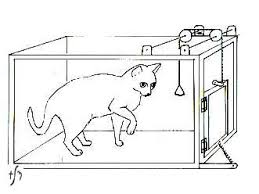
\includegraphics[scale=0.47]{slike/macka.jpg}
        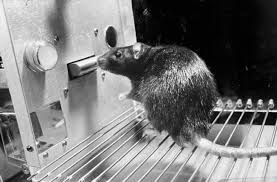
\includegraphics[scale=0.5]{slike/miska.jpg}
    \end{figure}
            
\end{frame}


\begin{frame}
    \frametitle{Okvir}
    \begin{figure}
        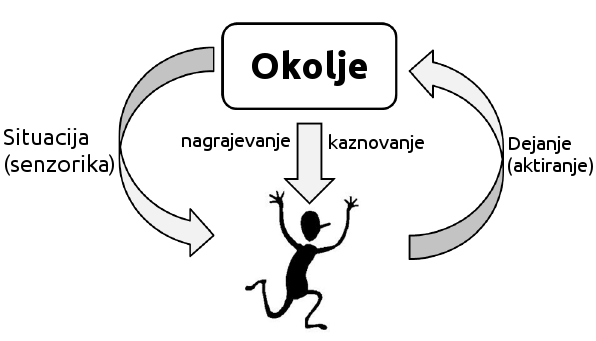
\includegraphics[scale=0.5]{slike/RLloop.png}
    \end{figure}
    \begin{itemize}
        \item Agent ">pade"< v okolje. 
        \item S poskušanjem se nauči pravilnih akcij.
        \item Svoje znanje izkoristi za maksimizacijo nagrade.
    \end{itemize}
\end{frame}


\begin{frame}[fragile]
    \frametitle{Primer: križci in krožci}
    \begin{columns}[T] % align columns
    \begin{column}{.48\textwidth}
    
    \begin{itemize}
        \item \textbf{Situacija/Stanje}: stanje na plošči,
        \item \textbf{Nagrada}: $1$ za zmago, $-1$ za poraz, $x$ za izenačenje/potezo,
        \item \textbf{Okolje}: nasprotnik, plošča, sodnik, nagrajevalec,
        \item \textbf{Akcija}: postavitev $X$ oz. $O$ na ploščo.
    \end{itemize}

    \end{column}%
    \hfill%
    \begin{column}{.48\textwidth}
    
        \begin{forest}
            TTT/.style args={#1:#2}{
              make tab/.expanded=\forestove{content},
              label={\pgfkeysvalueof{/forest/label position #1}:$#2$}
            },
            TTT*/.style={
              make tab=::/::/::,
              content/.expand once=%
              \expandafter\vphantom\expandafter{\romannumeral-`0\forestov{content}},
              draw=none,
              append after command={(\tikzlastnode.north) edge (\tikzlastnode.south)},
              for descendants={before computing xy={l*=1.2}},
            },
            th/.style=thick,
            for tree={node options=draw, inner sep=+0pt, parent anchor=south, child anchor=north}
            [o:x:o/x:x:/x:o:, TTT=r:
                [o:x:o/x:x:o/x:o:, TTT=b:
                    [o:x:o/x:x:o/x:o:x, TTT=b: x]
            ]
                [o:x:o/x:x:/x:o:o, TTT=b:
                    [o:x:o/x:x:x/x:o:o, TTT=b: 1]
            ]
            ]
        \end{forest}

    \end{column}%
    \end{columns}
\end{frame}


\begin{frame}
    \frametitle{Agent}
    Naj bo $\mathcal{S}$ množica vseh stanj, $\mathcal{A}$ množica vseh akcij, $S_t$, $R_t$ in $A_t$ pa 
    (slučajno) stanje, nagrada in akcija ob času $t$. 
    \medskip
    \medskip
    \pause

    Agent ima tri glavne komponente:
    \begin{itemize}
        \item Strategija (angl. \textit{Policy})
        \item Vrednostna funkcija (angl. \textit{Value function})
        \item Model
    \end{itemize}
    \end{frame}


\begin{frame}
    \frametitle{Agent: strategija}
    \begin{definicija}
        \begin{itemize}
            \item \textbf{Deterministična strategija} je preslikava $\pi: \mathcal{S} \rightarrow \mathcal{A}$, 
                    $$
                    \pi(s) = a.
                    $$ 
            \item \textbf{Stohastična strategija} je preslikava $\pi: \mathcal{A} \times 
                    \mathcal{S} \rightarrow [0, 1]$, 
                    $$
                    \pi(a | s) = P(A_t = a~|~S_t = s).
                    $$
        \end{itemize}
    \end{definicija}
\end{frame}


\begin{frame}
    \frametitle{Agent 3: vrednostna funkcija}
    \begin{definicija}[Povračilo]
        $$
        G_t = R_{t+1} + \gamma R_{t+2} + ... = \sum_{k=0}^\infty \gamma^k R_{t + k + 1}
        $$
    \end{definicija}
    \pause
    \begin{definicija}[Vrednostna funkcija]
        \begin{itemize}
            \item \textbf{Vrednostna funkcija stanja} je pogojno matematično upanje povračila, če začnemo v 
                    stanju $s$ in se nato vedemo skladno s strategijo $\pi$ 
                    $$
                    v_\pi(s) = \mathrm{E} [G_t~|~S_t = s].
                    $$
            \pause 
            \item \textbf{Vrednostna funkcija akcije} je podobna prejšnji, le da sprosti prvo akcijo 
                    $$
                    q_\pi(s, a) = \mathrm{E} [G_t~|~S_t = s, A_t = a].
                    $$
        \end{itemize}
    \end{definicija}
\end{frame}


\begin{frame}
    \frametitle{Formalizacija: Markovski proces odločanja 1}
    \begin{definicija}[Markovska veriga]
        Slučajni proces $(S_t)_{t=0}^T$ na končnem verjetnostnem prostoru 
        $(\Omega, \mathcal{F}, P)$ je \textbf{Markovska veriga}, če velja Markovska lastnost
        $$
        P(S_{t+1} = s_{t+1}~|~S_{t} = s_{t}, ..., S_0 = s_0) = P(S_{t+1} = s_{t+1}~|~S_{t} = s_{t})
        $$
    \end{definicija}
    \pause
    \medskip
    \begin{itemize}
        \item Prihodnost je neodvisna od preteklosti, če poznamo sedanjost
        \pause
        \item $p_{ss'} := P(S_{t+1} = s'~|~S_{t} = s) \rightarrow
                \mathcal{P} := [p_{ss'}]_{s,s'\in \mathcal{S} }$, 
        \pause
        \item \emph{Markovska veriga} je torej dvojica $(\mathcal{S}, \mathcal{P})$
    \end{itemize}
    
\end{frame}


\begin{frame}
    \frametitle{Formalizacija: Markovski proces odločanja 2}
    \begin{definicija}[Markovski proces nagrajevanja]
        \textbf{Markovski proces nagrajevanja} je nabor 
        $(\mathcal{S}, \mathcal{P}, \mathcal{R}, \gamma)$, kjer je
        \begin{itemize}
            \item $\mathcal{S}$ (končna) množica stanj,
            \item $\mathcal{P}$ prehodna matrika, kjer $\mathcal{P}_{ss'} = P(S_{t+1} = s'~|~S_{t} = s)$,
            \item $\mathcal{R}$ nagradna funkcija $\mathcal{R}_s = E[R_{t+1}~|~S_{t} = s]$,
            \item $\gamma \in [0, 1]$ je diskontni faktor.
        \end{itemize}
    \end{definicija}
\end{frame}


\begin{frame}
    \frametitle{Formalizacija: Markovski proces odločanja 3}
    \begin{definicija}[Markovski proces odločanja]
        \textbf{Markovski proces odločanja (MDP)} je nabor 
        $(\mathcal{S}, \mathcal{A}, \mathcal{P}, \mathcal{R}, \gamma)$, kjer je
        \begin{itemize}
            \item $\mathcal{S}$ (končna) množica stanj,
            \item $\mathcal{A}$ (končna) množica akcij oz. dejanj,
            \item $\mathcal{P}$ prehodna matrika, kjer $\mathcal{P}_{ss'}^a = P(S_{t+1} = s'~|~S_{t} = s,
                    \mathbf{A_t = a})$,
            \item $\mathcal{R}$ nagradna funkcija $\mathcal{R}_s^a = E[R_{t+1}~|~S_{t} = s, 
                    \mathbf{A_t = a}]$,
            \item $\gamma \in [0, 1]$ diskontni faktor.
        \end{itemize}
    \end{definicija}
\end{frame}


\begin{frame}
    \frametitle{Algoritmi}
    \begin{itemize}
        \item Učenje prek strategije ali \textbf{vrednostne funkcije}. 
        \item Celoten problem je \textbf{načrtovanje}:
        \begin{itemize}
            \item Napovedovanje - ugotvaljanje vrednosti.
            \item Upravljanje - iskanje optimalne strategije. 
        \end{itemize}
    \end{itemize}
\end{frame}


\begin{frame}
    \frametitle{Algoritmi: dinamično programiranje}
    Bellmanova enačba pričakovanja:
        \begin{align*}
            v_\pi(s) = \mathrm{E} [G_t~|~S_t = s] &= \dots = \mathrm{E} [R_{t+1} + \gamma v_\pi(S_{t+1})~|~S_t = s], \\
            v_\pi &= \mathcal{R}^\pi + \gamma \mathcal{P}^\pi v_\pi, \\
            v_{k+1} &= \mathcal{R}^\pi + \gamma \mathcal{P}^\pi v_k.
        \end{align*}
        \only<1>{
    \begin{izrek}
        Za vsak končni Markovski proces odločanja s končnimi nagradami velja: 
        \begin{enumerate}
            \item Obstaja \textit{optimalna} strategija $\pi_*$, ki je boljša 
                    ali enaka kot vse ostale strategije; $\pi_* \geq \pi \text{ za vsak }  \pi \in \Pi$. 
            
            \item Vedno obstaja optimalna strategija, ki je \textit{deterministična}.
    
            \item Vse optimalne strategije določajo enako optimalno vrednostno funkcijo stanja in 
                    optimalno vrednostno funkcijo akcije:
                    \begin{align*}
                        v_{\pi*}(s) &= v_*(s), \\
                        q_{\pi*}(s, a) &= q_*(s, a).
                    \end{align*}
        \end{enumerate} 
    \end{izrek}
        }
    \only<2>{
        \begin{figure}
            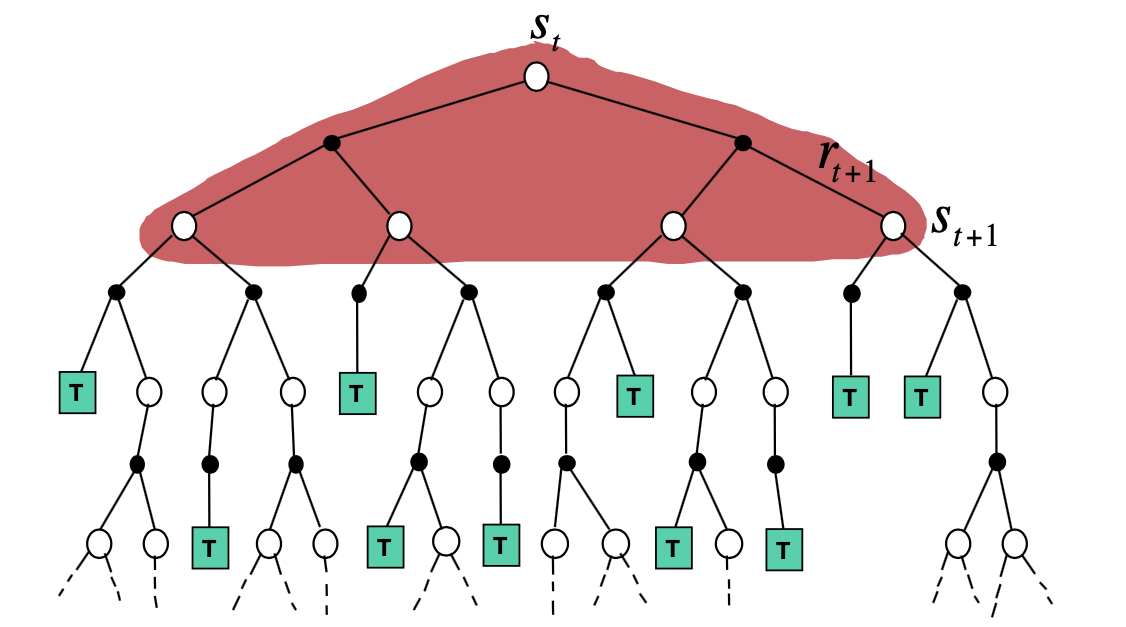
\includegraphics[scale=0.47]{slike/backup-dp.png}
        \end{figure}
    }
\end{frame}


\begin{frame}
    \frametitle{Algoritmi: Monte Carlo 1}
    \begin{itemize}
        \item Nepoznan epizodični MDP, 
        \item problem napovedovanja, 
        \item empirično povračilo, 
        \item štejemo obiske stanj.
    \end{itemize}
\end{frame}


\begin{frame}
    \frametitle{Algoritmi: Monte Carlo 2}
    \begin{itemize}
        \item Ob \textbf{vsakem} obisku stanja $s$: 
        \begin{align*}
            N(s) &\leftarrow N(s) + 1 \\
            S(s) &\leftarrow S(s) + G_t
        \end{align*}
        \item Po koncu učenja: 
        $$
        V(s) \leftarrow S(s) / N(s)
        $$
        \pause
       \item Pomni: Računanje povprečja zaporedja $(X_i)_{i \in \mathbb{N}}$
       $$
       \mu_k = \frac{1}{k} \sum_{j=1}^k X_j = \mu_{k-1} + \frac{1}{k} (X_k - \mu_{k-1})
       $$
       \pause
       \item Inkrementalni Monte Carlo:
       $$
       V(S_t) \leftarrow V(S_t) + \frac{1}{N(S_t)} (G_t - V(S_t))
       $$
    \end{itemize}
\end{frame}


\begin{frame}
    \frametitle{Algoritmi: Monte Carlo 3}
    \begin{itemize}
        \item Inkrementalni Monte Carlo:
                %$$
                %V(s) \leftarrow V(s) + \alpha (G_t - V(S_t)).
                %$$
                \begin{figure}[b]
                    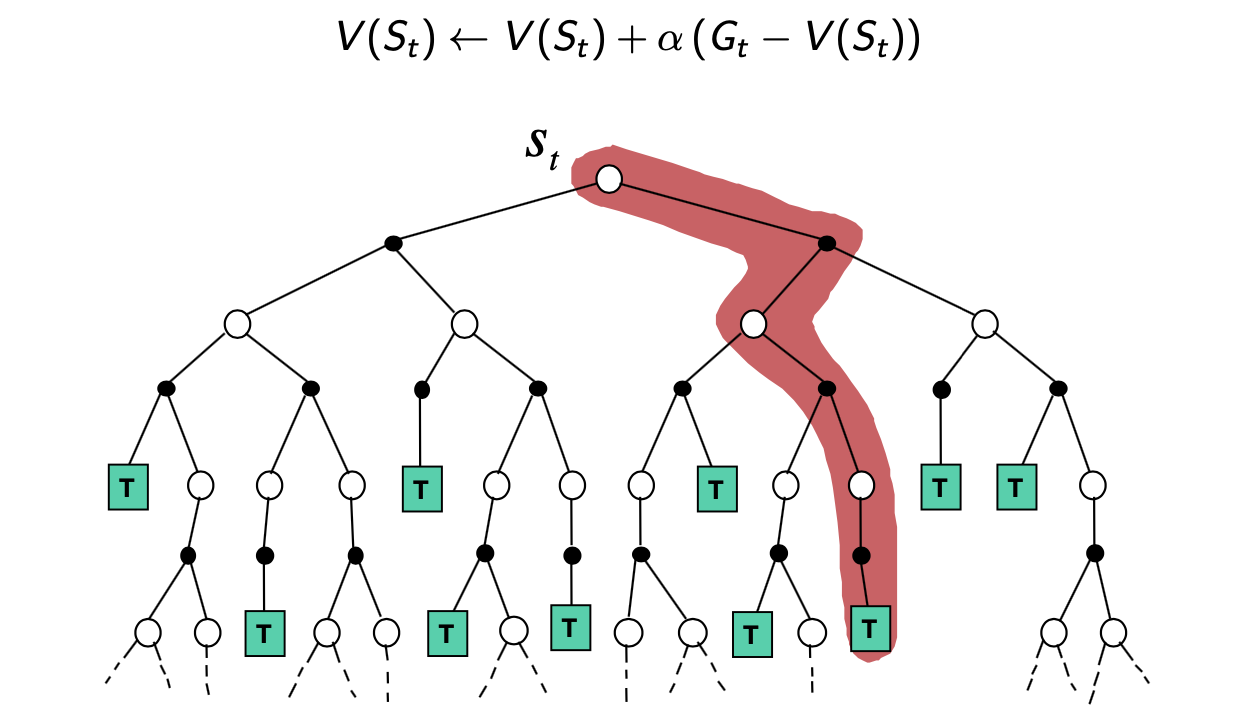
\includegraphics[scale=0.45]{slike/backup-mc.png}
                \end{figure}
        \item Splošni obrazec: 
                $$
                \textit{nova ocena} \leftarrow \textit{stara ocena} + \textit{korak } 
                (\textit{tarča} - \textit{stara ocena}).
                $$
    \end{itemize}
\end{frame}


\begin{frame}
    \frametitle{Algoritmi: TD($0$)}
    \begin{itemize}
        \item Učenje s časovno razliko.
        \item \textit{Bootstrapping}. 
        \item Ne potrebujejo povračila.
        \item $G_t \approx R_{t+1} + \gamma V(S_{t+1})$.
    \end{itemize}

    %\medskip
    %$$
    %V(S_t) \leftarrow V(S_t) + \alpha (R_{t+1} + \gamma V(S_{t+1}) - V(S_t)).
    %$$
    \begin{figure}[b]
        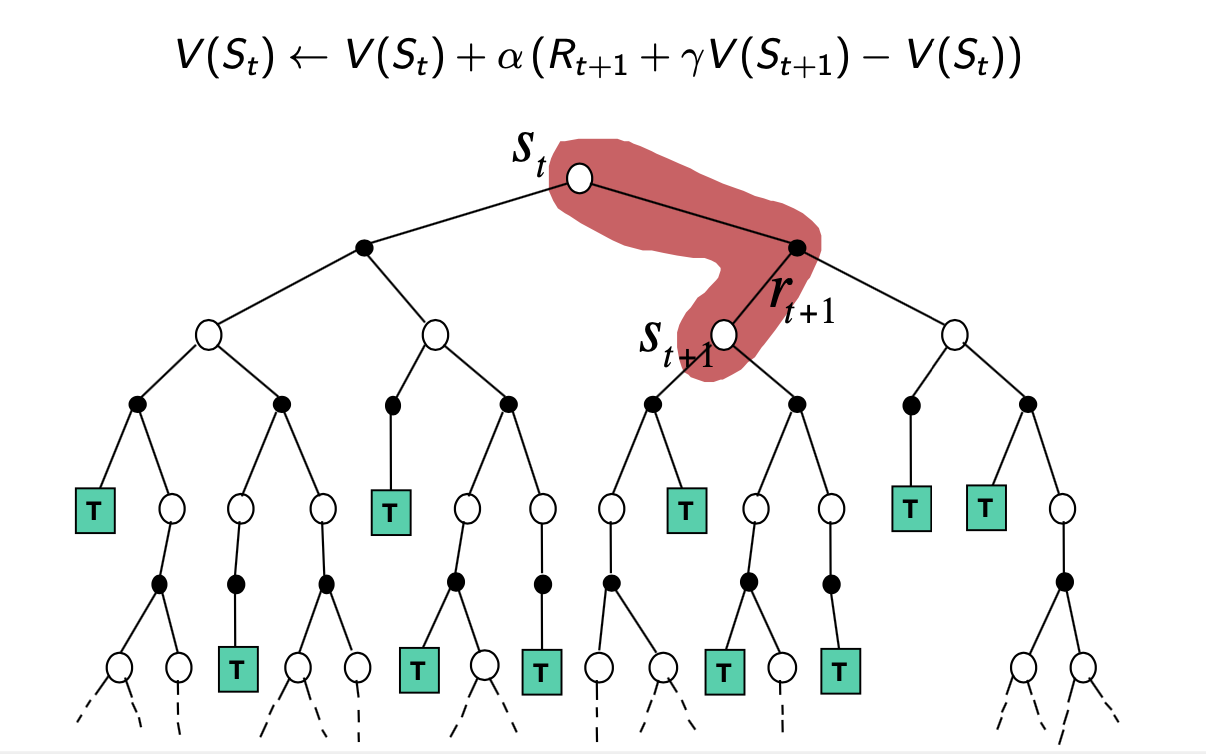
\includegraphics[scale=0.45]{slike/backup-td.png}
    \end{figure}
\end{frame}


\begin{frame}
    \frametitle{Algoritmi: TD($\lambda$) 1}
    \begin{itemize}
        \item Povezava med MC in TD($0$).
        \item $G_t^{(n)} = R_{t+1} + \dots + \gamma^{n-1} R_{t+n} + \gamma^n V(S_{t+n}).$
        \item Povprečenje različnih $G_t^{(n)}$: $G_t^\lambda = (1 - \lambda) \sum_{n=1}^\infty 
                                                 \lambda^{(n-1)} G_t^{(n)}.$
    \end{itemize}

    \medskip
    \medskip
    \medskip
    \pause
    TD($\lambda$) s \textbf{pogledom naprej}: 
    $$
    V(S_t) \leftarrow V(S_t) + \alpha (G_t^\lambda - V(S_t)).
    $$
    \begin{figure}[b]
        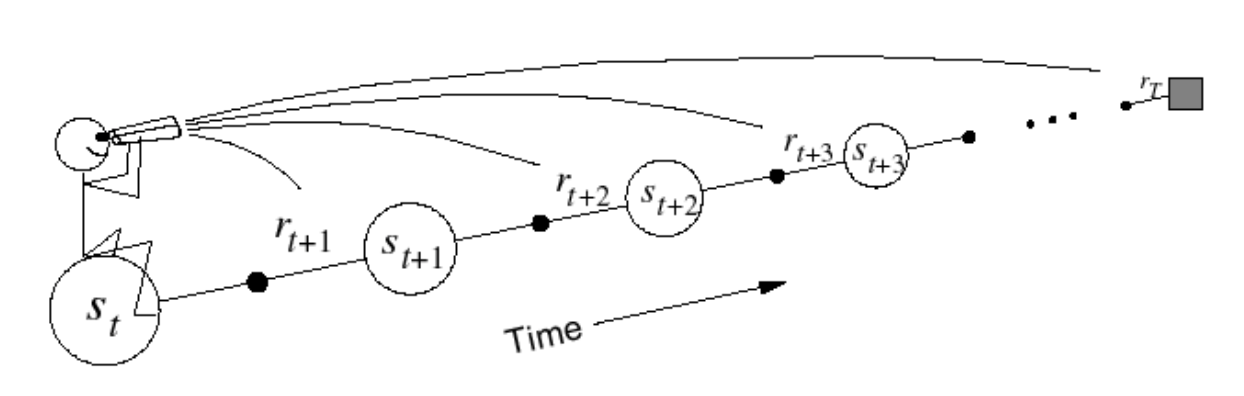
\includegraphics[scale=0.45]{slike/pogled-naprej.png}
    \end{figure}
\end{frame}


\begin{frame}
    \frametitle{Algoritmi: TD($\lambda$) 2}
    \begin{itemize}
        \item \textbf{Sledi upravičenosti} (angl. \textit{eligibility traces}):
        \begin{align*}
            E_0(s) &= 0, \\
            E_t(s) &= \gamma \lambda E_{t-1}(s) + \mathbbm{1}(S_t = s),
        \end{align*}
    \begin{figure}
        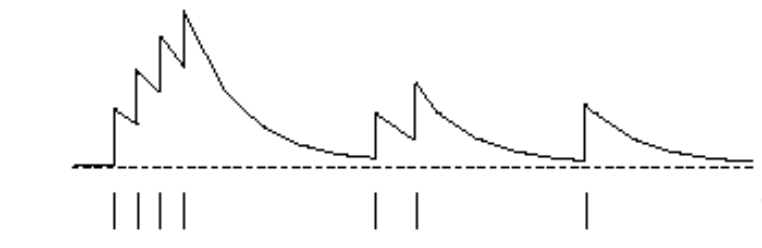
\includegraphics[scale=0.25]{slike/et.png}
    \end{figure}
        \pause
        \item $\delta_t = R_{t+1} + \gamma V(S_{t+1}) - V(S_t).$
    \end{itemize}

    \medskip
    \medskip
    \medskip
    TD($\lambda$) s \textbf{pogledom nazaj}: 
    $$
    V(s) \leftarrow V(s) + \alpha \delta_t E_t(s).
    $$
    \begin{figure}[b]
        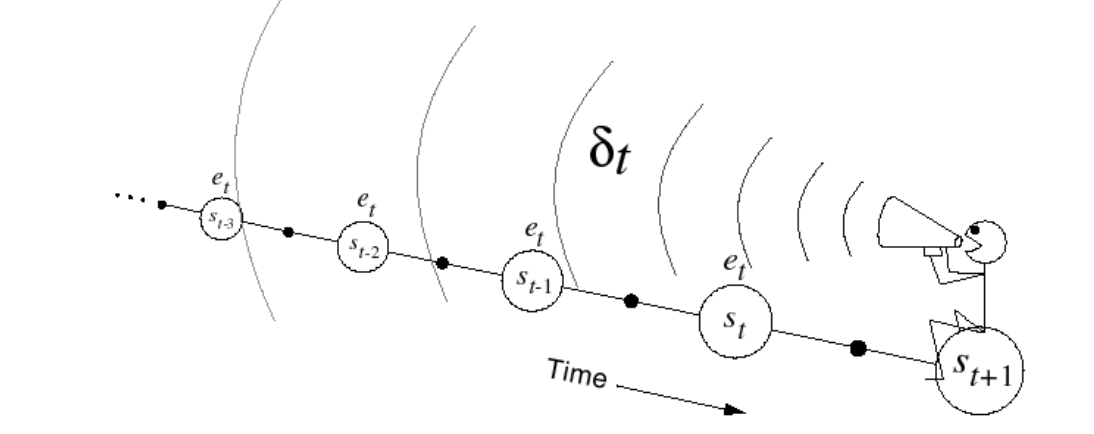
\includegraphics[scale=0.35]{slike/pogled-nazaj.png}
    \end{figure}
\end{frame}


\begin{frame}
    \frametitle{Spreminjanje strategije - upravljanje}
    \begin{figure}
        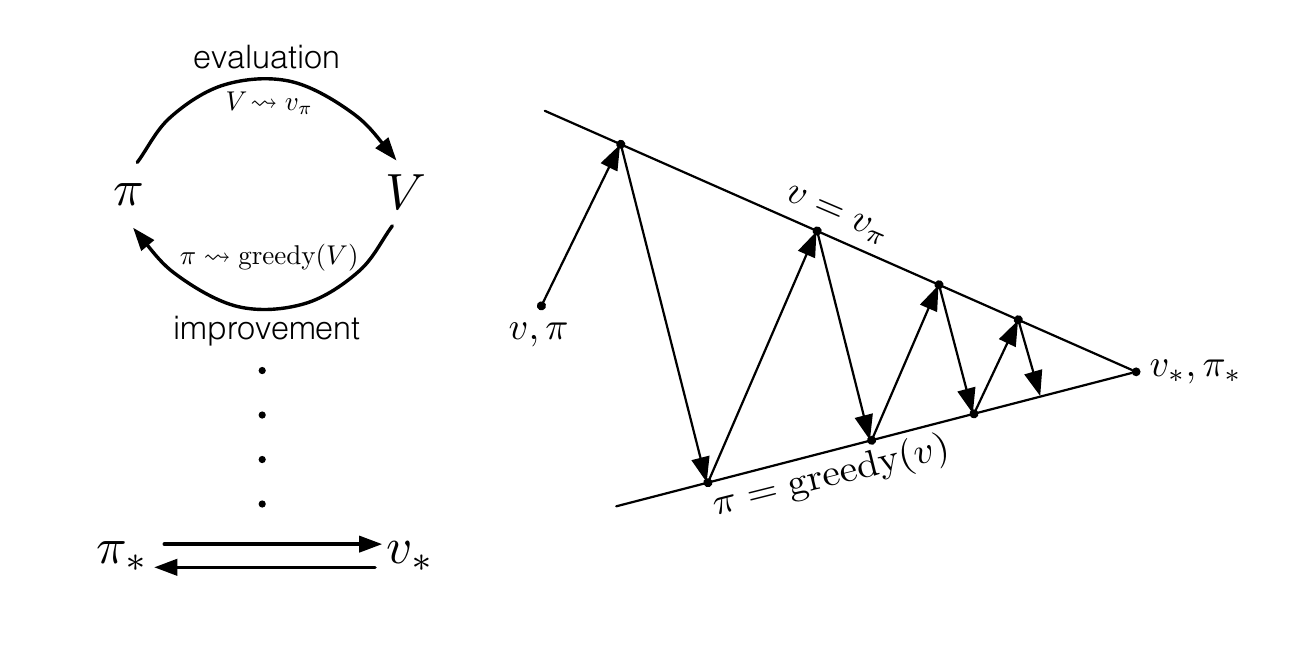
\includegraphics[scale=0.2]{slike/policy-iteration.png}
    \end{figure}
    \pause
    \begin{itemize}
        \item Potrebujemo vrednostno funkcijo akcij. 
        \item Raziskovanje in izkoriščanje.
        \item $\epsilon$-požrešna izbira akcij:
        \begin{equation*}
            \pi'(a|s) = \begin{cases}
                \epsilon / m + 1 - \epsilon & \text{če } a = \text{arg}\max_{a \in 
                    \mathcal{A}} q_\pi(s, a), \\
                    \epsilon / m & \text{sicer},
               \end{cases}
        \end{equation*}
    \end{itemize}
\end{frame}


\begin{frame}
    \frametitle{Primer algoritma}
    \begin{algorithm}[H]
        \caption{SARSA}
    \begin{algorithmic}\label{SARSA}
        
        \STATE \textbf{Podatki}: parameter hitrosti učenja $\alpha$, število epizod $stEpizod$, diskontni 
                faktor $\gamma$, parameter požrešnosti $\epsilon$
        \STATE Poljubno nastavimo vrednosti $Q(s, a)$ za vsak $s \in \mathcal{S}$ in $a \in \mathcal{A}$ 
        \FOR{$k = 1, 2, \dots, stEpizod$}
            \STATE Generiraj epizodo prek funkcije $Q$ $\epsilon$-požrešno
            \STATE $stanja \leftarrow$ seznam vseh opaženih stanj
            \STATE $nagrade \leftarrow$ seznam vseh opaženih nagrad
            \STATE $akcije \leftarrow$ seznam vseh opaženih akcij
            \FOR{$t = 1, 2, \dots, length(stanja)$}
            \STATE $s = stanja[t]$
            \STATE $s' = stanja[t + 1]$
            \STATE $a = akcije[t]$
            \STATE $a' = akcije[t + 1]$
            \STATE $Q(s, a) \leftarrow Q(s, a) + \alpha (nagrade[s'] + \gamma Q(s', a') - Q(s, a))$ 
            \ENDFOR
        \ENDFOR
    
    \end{algorithmic}
    \end{algorithm}
\end{frame}


\begin{frame}
    \frametitle{Konvergenca}
    \textbf{PLNR}:
    \begin{itemize}
        \item Vsi pari stanj in akcij so obiskani oz. uporabljeni neskončnokrat.
        \item Zaporedje strategij konvergira proti požrešni, torej 
            $$
            \lim_{k \rightarrow \infty} \pi_k(a|s) = \mathbbm{1} (a = \text{arg}\max_{a \in \mathcal{A}} 
                q(s, a)).
            $$
    \end{itemize}
    \begin{izrek}
        Algoritem SARSA konvergira proti optimalni vrednostni funkciji akcij $q_*$, če veljata naslednja 
        pogoja:
        \begin{itemize}
            \item Zaporedje strategij je PLNR (npr. $\epsilon$-požrešno z $\epsilon_k = 1 / k$).
            \item Zaporedje parametrov hitrosti učenja $\alpha_k$ zadošča pogojema
                $$
                \sum_{k=1}^\infty \alpha_k = \infty~\text{ in }~\sum_{k=1}^\infty \alpha_k^2 < \infty.
                $$
        \end{itemize}
    \end{izrek}
\end{frame}


\begin{frame}
    \frametitle{Aproksimacija}
    \begin{itemize}
        \item Veliki MDP-ji 
                \begin{itemize}
                    \item križci in krožci: $3^9$ / $4578$ / $765$ stanj, 
                    \item štiri v vrsto: $4.531.985.219.092$ stanj,
                    \item šah: približno $10^{46}$ stanj, 
                    \item go: $10^{170}$ stanj, 
                \end{itemize}
        \medskip
        \medskip
        \item Vsi zgornji algoritmi so tabelarični.
        \item $\hat{v}(s, w) \approx v_\pi(s)$ oz. $\hat{q}(s, a, w) \approx q_\pi(s, a)$
        \item Linearna aproksimacija ali nevronske mreže
        \item Konvergenca?
    \end{itemize}
\end{frame}


\begin{frame}
    \frametitle{Gradientni spust}
    \begin{itemize}
        \item Premikamo se proti minimumu funkcije $J$, 
            $$
            \Delta w = - \alpha \nabla_wJ(w).
            $$
        \item V našem primeru srednja kvadratična napaka
            \begin{align*}
                J(w) &= E_\pi [(v_\pi(s) - \hat{v}(s, w))^2], \\
                \Delta w &= \alpha E_\pi [(v_\pi(s) - \hat{v}(s, w)) \nabla_w \hat{v}(s, w)].
            \end{align*}
        \item Ker ne poznamo okolja, vzorčimo
            $$
            \Delta w = \alpha (v_\pi(s) - \hat{v}(s, w)) \nabla_w \hat{v}(s, w).
            $$
        \item Algoritem TD($\lambda$) je potem 
            $$
            \Delta w = \alpha (G_t^\lambda - \hat{v}(s, w)) \nabla_w \hat{v}(s, w).
            $$
    \end{itemize}
\end{frame}


\begin{frame}
    \frametitle{Namizne igre}
    \begin{itemize}
        \item Kombinatorne igre: dva igralca, popolna informacija, izmenične poteze,
        \item Enostavno nagrajevanje,
        \item ">po-stanja"<,
        \item Pridobivanje iger: 
                \begin{itemize}
                    \item Nasprotnik iz podatkovne baze, 
                    \item naključni nasprotnik,
                    \item fiksiran nasprotnik, 
                    \item samoigra.
                \end{itemize}
        \item Gledamo skupno strategijo $\pi = (\pi_1, \pi_2)$ in minimax vrednostno funkcijo
        $$
        v_*(s) = \max_{\pi_1} \min_{\pi_2} v_\pi(s).
        $$
    \end{itemize}
\end{frame}


% FRAME KJER OPIŠEŠ POSTOPEK??????


\begin{frame}
    \frametitle{Rezultati}
    \begin{columns}
        \begin{column}{5.5cm}
            \begin{itemize}
                \item<1-> $3$,$3$,$3$-igra in tabelarični agent
                \item<2-> $3$,$3$,$3$-igra in agent z nevronsko mrežo
                \item<3-> $5$,$5$,$4$-igra in tabelarični agent
                \item<4-> $5$,$5$,$4$-igra in agent z nevronsko mrežo
            \end{itemize}
        \end{column}

        \begin{column}{6.5cm}
            \only<1>{
                \begin{figure}
                    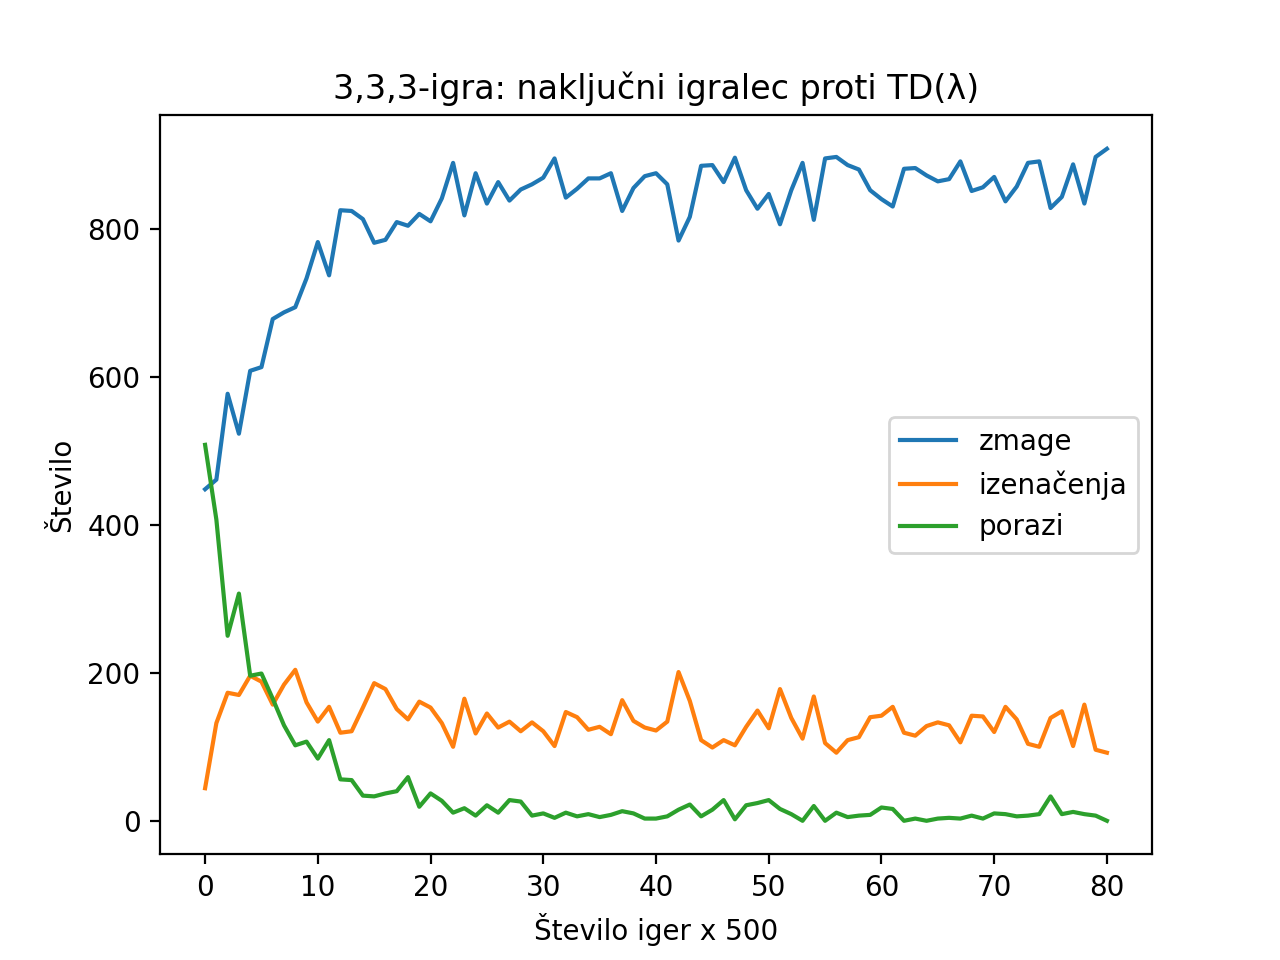
\includegraphics[width=6.5cm]{../../rezultati/tdl-333-40000-2.png}
                \end{figure}
            }
            \only<2>{
                \begin{figure}
                    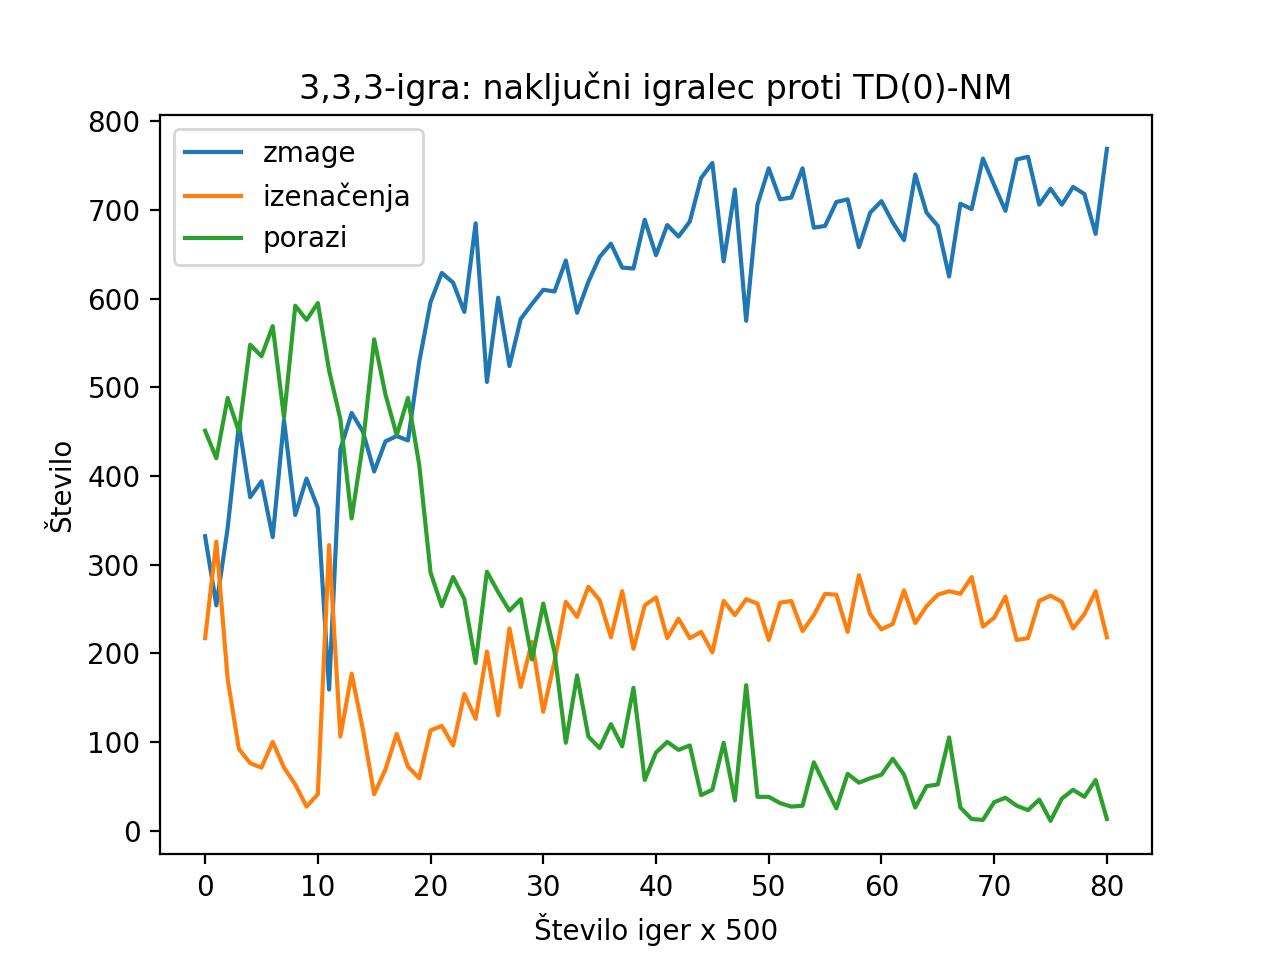
\includegraphics[width=6.5cm]{../../rezultati/tdnn-333-40000-2.png}
                \end{figure}
            }
            \only<3>{
                \begin{figure}
                    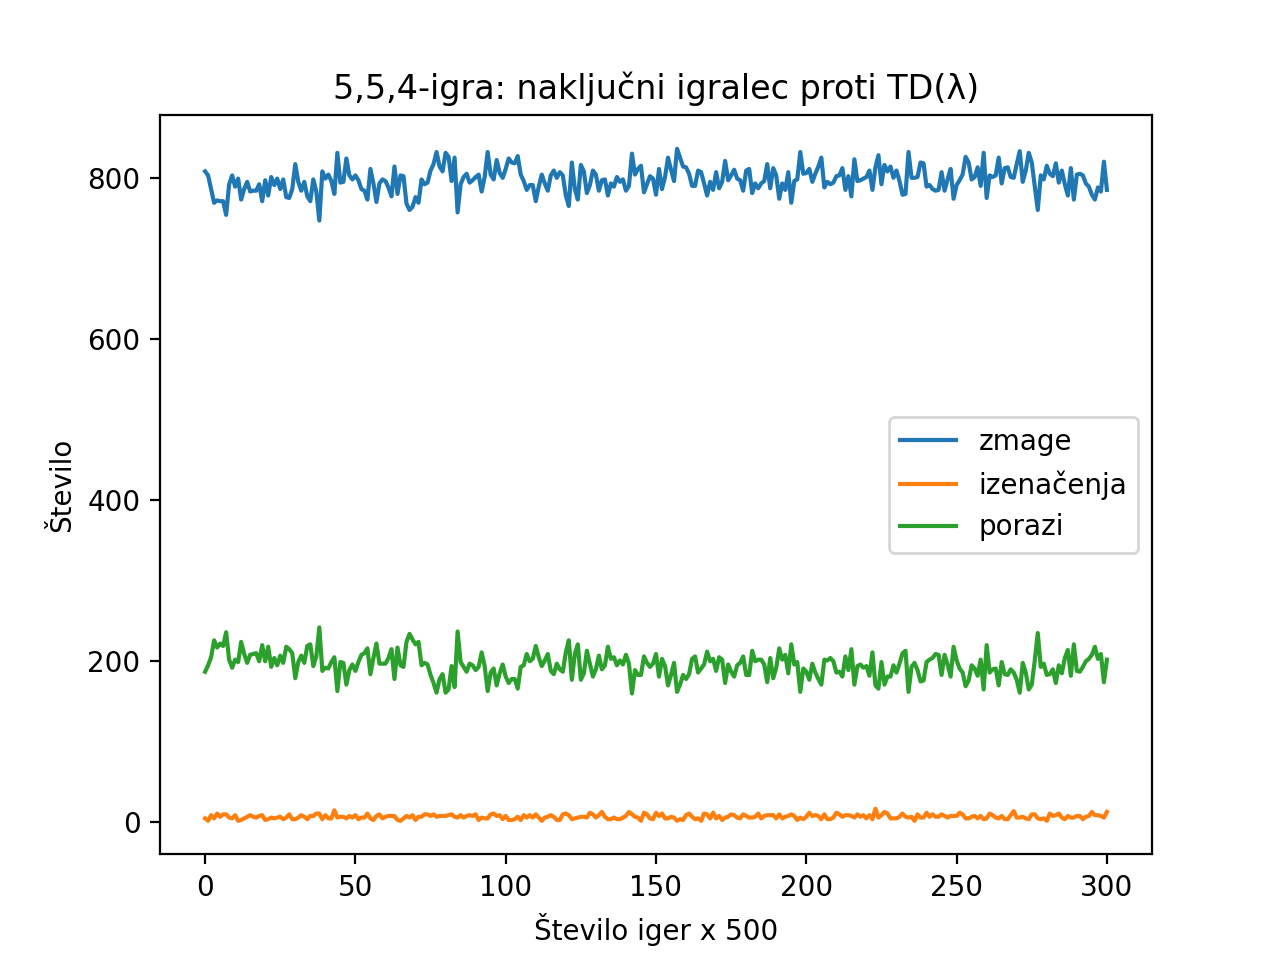
\includegraphics[width=6.5cm]{../../rezultati/tdl-554-150000-2.png}
                \end{figure}
            }
            \only<4>{
                \begin{figure}
                    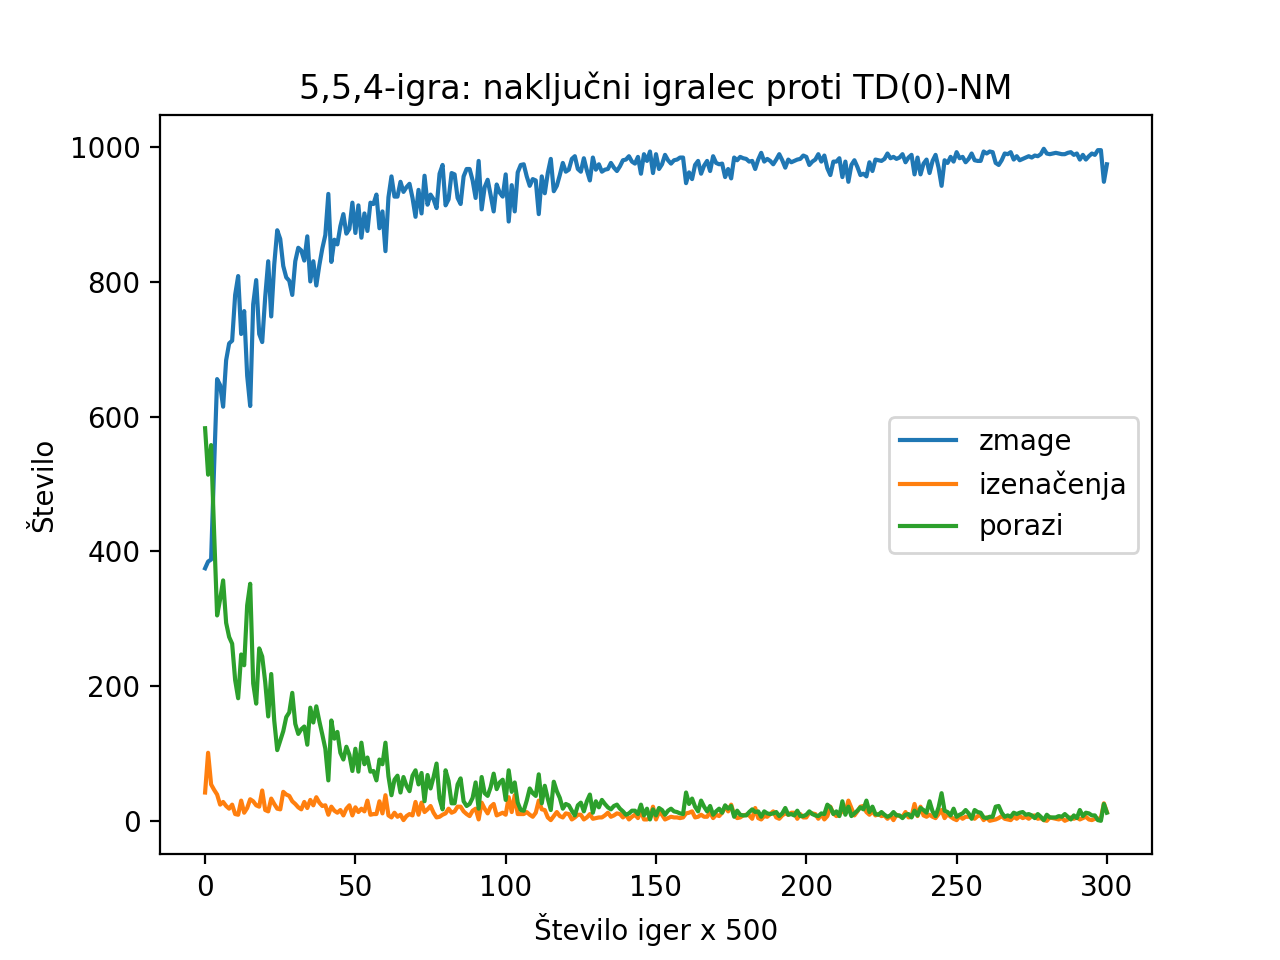
\includegraphics[width=6.5cm]{../../rezultati/tdnn-554-150000-2.png}
                \end{figure}
            }
        \end{column}
    \end{columns}
\end{frame}


\begin{frame}[t, allowframebreaks]
    \frametitle{Literatura}
    \nocite{*}
    \fontsize{6pt}{0pt}
    \begin{thebibliography}{10}

        \bibitem{DP}
        R.~E. Bellman.
        \newblock {\em Dynamic Programming}.
        \newblock Princeton University Press, Princeton, 1957.
        
        \bibitem{MDP}
        R.~E. Bellman.
        \newblock A markov decision process.
        \newblock {\em Journal of Mathematical Mechanics}, 6, 1957.
        
        \bibitem{RLboard}
        I.~Ghory.
        \newblock Reinforcement learning in board games,
        \newblock 2004.
        
        \bibitem{SSA}
        A.~W. Hales in R.~I. Jewett.
        \newblock Regularity and positional games.
        \newblock {\em Transactions of the American Mathematical Society}, 106, 1963.
        
        \bibitem{NN}
        K.~Hornik, M.~Stinchcombe in H.~White.
        \newblock Multilayer feedforward networks are universal approximators.
        \newblock {\em Neural networks}, 2, 1989.
        
        \bibitem{LecNotesSilver}
        D.~Silver.
        \newblock Introduction to reinforcement learning.
        \newblock
          \url{https://deepmind.com/learning-resources/-introduction-reinforcement-learning-david-silver},
          2015.
        
        \bibitem{go}
        D.~Silver~idr.
        \newblock Mastering the game of go with deep neural networks and tree search.
        \newblock {\em Nature}, 529, 2016.
        
        \bibitem{dokaz}
        S.~Singh, T.~Jaakkola, M.~L. Littmanm in C.~Szepesvari.
        \newblock Convergence results for single-step on-policy reinforcement-learning
          algorithms.
        \newblock {\em Machine Learning}, 39, 2000.
        
        \bibitem{MCdokaz}
        S.~Singh in R.~S. Sutton.
        \newblock Reinforcement learning with replacing eligibility traces.
        \newblock {\em Machine Learning}, 22, 1996.
        
        \bibitem{TDlambda}
        R.~S. Sutton.
        \newblock Learning to predict by the methods of temporal differences.
        \newblock {\em Machine Learning}, 3, 1988.
        
        \bibitem{RLintro}
        R.~S. Sutton in A.~G. Barto.
        \newblock {\em Reinforcement Learning: An introduction}.
        \newblock The MIT Press, Cambridge, Massachusetts, 2 edition, 2015.
        
        \bibitem{RLalgo}
        C.~Szepesvari.
        \newblock {\em Algorithms for Reinforcement Learning}.
        \newblock Morgan \& Claypool Publishers, Alberta, Canada, 2009.
    
        \bibitem{github}
        \emph{The Agent-Environment Interaction figure from Reinforcement Learning: An Introduction by Richard S. Sutton and Andrew G. Barto reproduced in Tikz}, v: GitHub, [ogled 5.~8.~2021], dostopno na \url{https://gist.github.com/pierrelux/6501790}.
    
        \bibitem{so}
        \emph{Creating Tic-Tac-Toe boards with LaTeX/TikZ}, v: TeX - LaTeX Stack Exchange, [ogled 12.~9.~2021], dostopno na \url{https://tex.stackexchange.com/questions/139782/creating-tic-tac-toe-boards-with-latex-tikz}.
    
        \end{thebibliography}
\end{frame}

\end{document}